% Created:  
% Author:   Julie Sewards
% Filename: implementation.tex

\chapter{Implementation}
\label{cha:imp}
\section{Development Environment}
An early challenge encountered in this project was setting up a suitable development environment.  Initially the intention was to use the Android Development Tools plug-in for Eclipse, as this was an extension to an already familiar IDE, however, difficulties were encountered with the school computers and finally we elected to switch to Android Studio (Beta) as suggested on the Android Developers website \citep{androiddev}.  

Since the main rationale for the Android application was to allow users to read documents away from the PC, we felt that the application should be optimised for use on a tablet.  As a difficulty arose in getting the device emulators to work on Linux, it became necessary to purchase a physical device for the purposes of the project.  Budget too was a significant consideration; therefore the device chosen was a Hudl 7" tablet running the Android 4.2.2 Jelly Bean operating system.  For the purposes of this project, it was decided that we would develop and test for this device.  This meant that we were restricted to API 17, which eliminated the need to include any backward compatibility but also precluded using features of the latest Android releases as it transpired that there was no upgrade path available for this device.  This fact turned out to be highly significant in a later stage of the project.  

\section{Initial Development}
It was felt wise to begin by developing a very simple application in order to gain some familiarity with the complexities of the Android architecture and its API. This initial application enabled us to input some text, encrypt it (using "convert to upper case" in lieu of encryption) and write it to the application storage.  

The next stage was to introduce actual encryption, for which we needed to investigate the Java Cryptography Architecture(JCA).  Although the choice of algorithm was determined as part of the design, we were mindful of the fact that  many security weaknesses are introduced by poor implementation. As \citet{schneier1998security} states,
\begin{quotation}
'And just as it's possible to build a weak structure using strong materials, it's possible to build a weak cryptographic system using strong algorithms and protocols' 
\end{quotation}  
For this reason we decided that we would initially develop and test the  Java classes to be used for encryption and decryption in the more familiar Linux environment before porting to Android.  Linux also provides a simple command line interface which was valuable for inspecting the binary (or hex) content of encrypted files to aid debugging.

\section{SecurelyShare Prototype}
In undertaking this project we were keen to understand more of the tools and techniques of Android development, therefore we attempted to incorporate a number different user interface components including altert and custom dialogs, fragments and ActionBar menus.
\subsection*{Initialisation}

The Initialisation Activity is run the first time SecurelyShare is installed.  The user is asked whether they wish to import a KeyStore from backup and asked to set up a master password.  In the current implementation, the import option must be chosen as the Certificate keystore needs to be created on a PC, either in Linux using  \texttt{keytool} from the command line or using a program called \texttt{Portecle}  \citep{portecle}.  An empty keystore is created for the group keys and the user is asked to confirm to proceed.  We used 

\begin{figure}[h!]
    \centering
    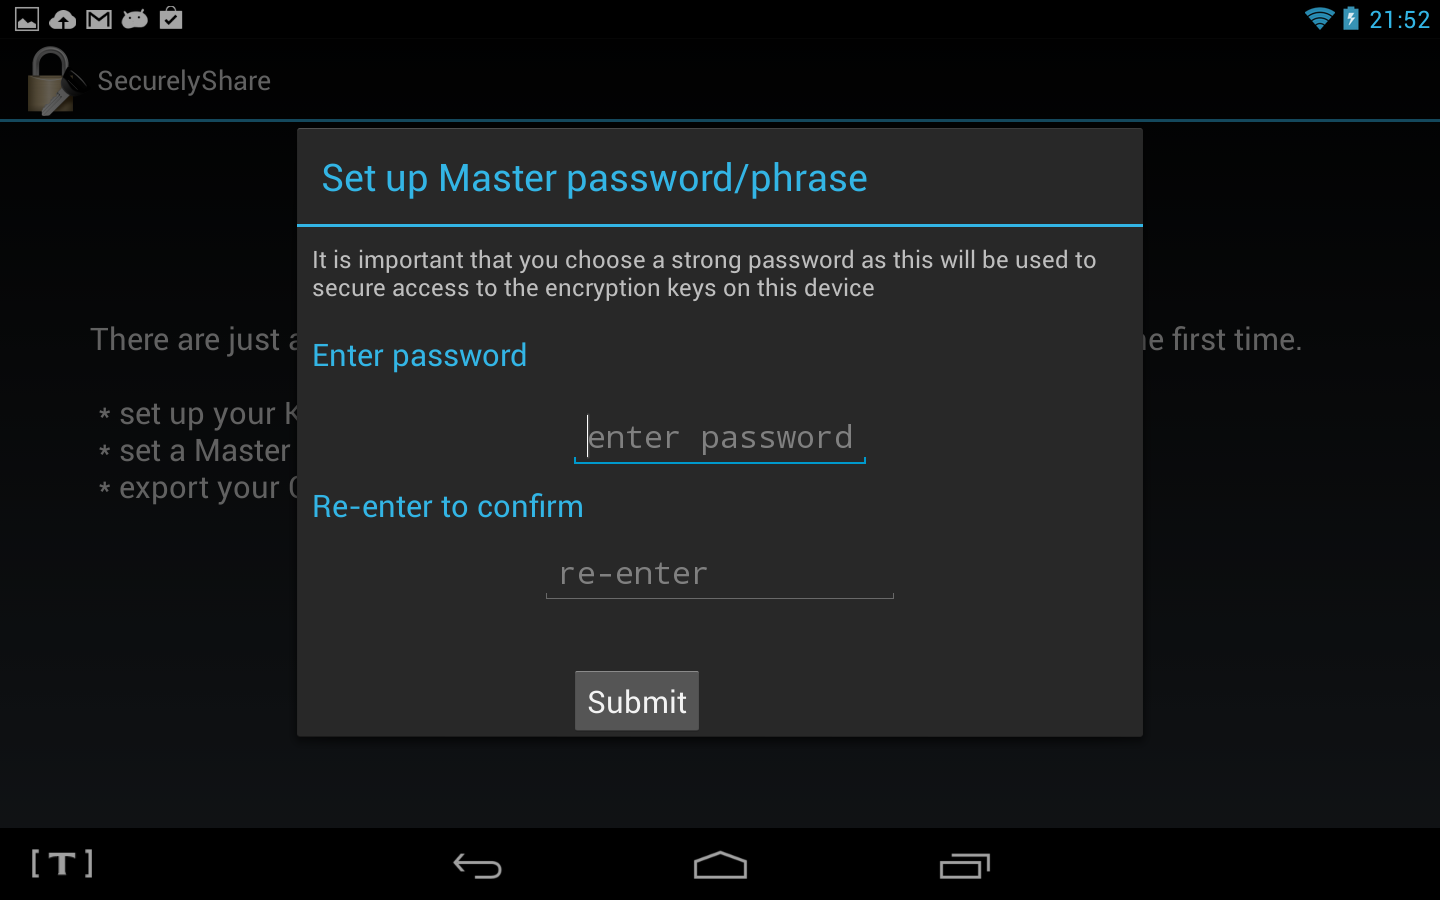
\includegraphics[width=0.6\textwidth]{Setup}                                                                                                                                                                                                                                                                                                                                                                                                                                                                                                                                                                                                                                                                                                                                                                                                                                                                                                                                                                                                                                                                                                                                                                                                                                                                                                                                                                                                                                                                                                                                                                                                                                                                                                                                                                                                                                                                                                                                                                                                                                                                                                                                                                                                                                                                                                                                                                                                                                                                                                                                                                                                                                                                                                                                                                                                                                                                                                                                                                          
    \caption{Set Master Password }
    \label{fig:alert}
\end{figure}

\subsection*{Main Activity}
The home page consists simply of four buttons for loving to the other main activities in SecurelyShare.  We recognise that this is somewhat visually unappealing and duplicates the menu options included in the Action Bar, however, in line with our design goals, it was felt better to focus on improving security features rather than visual appeal at this stage.

\begin{figure}[h!]
    \centering
    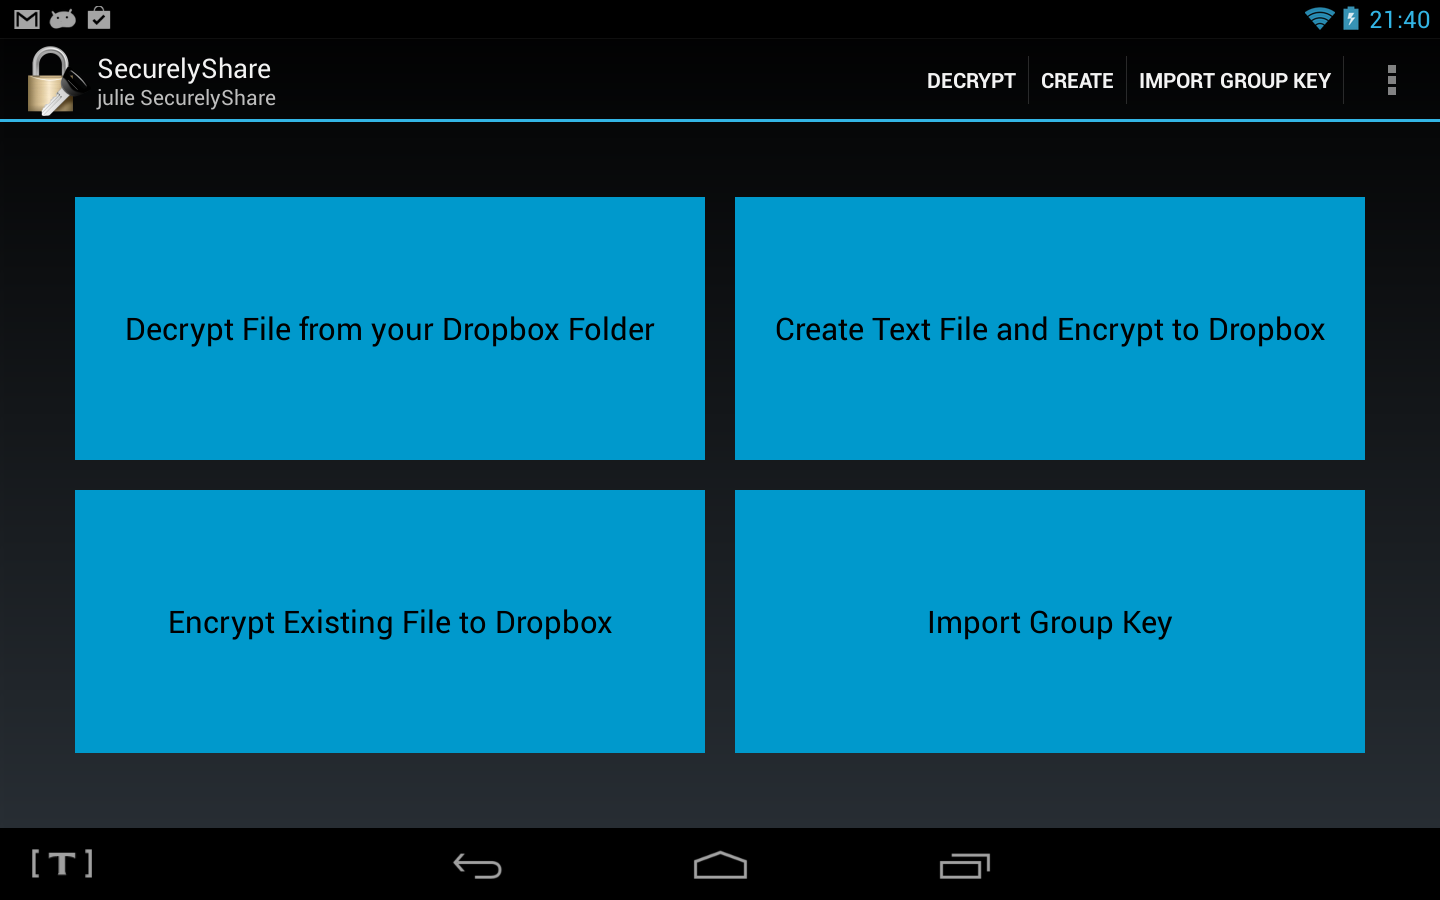
\includegraphics[width=0.6\textwidth]{main}                                                                                                                                                                                                                                                                                                                                                                                                                                                                                                                                                                                                                                                                                                                                                                                                                                                                                                                                                                                                                                                                                                                                                                                                                                                                                                                                                                                                                                                                                                                                                                                                                                                                                                                                                                                                                                                                                                                                                                                                                                                                                                                                                                                                                                                                                                                                                                                                                                                                                                                                                                                                                                                                                                                                                                                                                                                                                                                                                                          
    \caption{Basic home screen}
    \label{fig:main}
\end{figure}

The user is invited to enter the Master password upon opening the application and, having decided that we would not require the password to be re-entered to access each file, it was necessary to ensure that this data was available wherever needed. Although the option of writing the password to the  \texttt{SharedPreference} database, from whence it could be accessed by other activities, would have been an easy solution, we did not feel that this represented good practice.  Further research revealed this to be a contentious question, with experienced developers divided as to whether this was best done by extending the \texttt{Application} class or by use of the Singleton design pattern.  As the guidance from Android Developers website states that 'there is normally no need to subclass Application. In most situation, static singletons can provide the same functionality in a more modular way'   \citep{androiddev2} , we decided to use this approach but recognise we may not have completely understood the full complexities of this problem at this juncture.

\begin{figure}[h!]
    \centering
    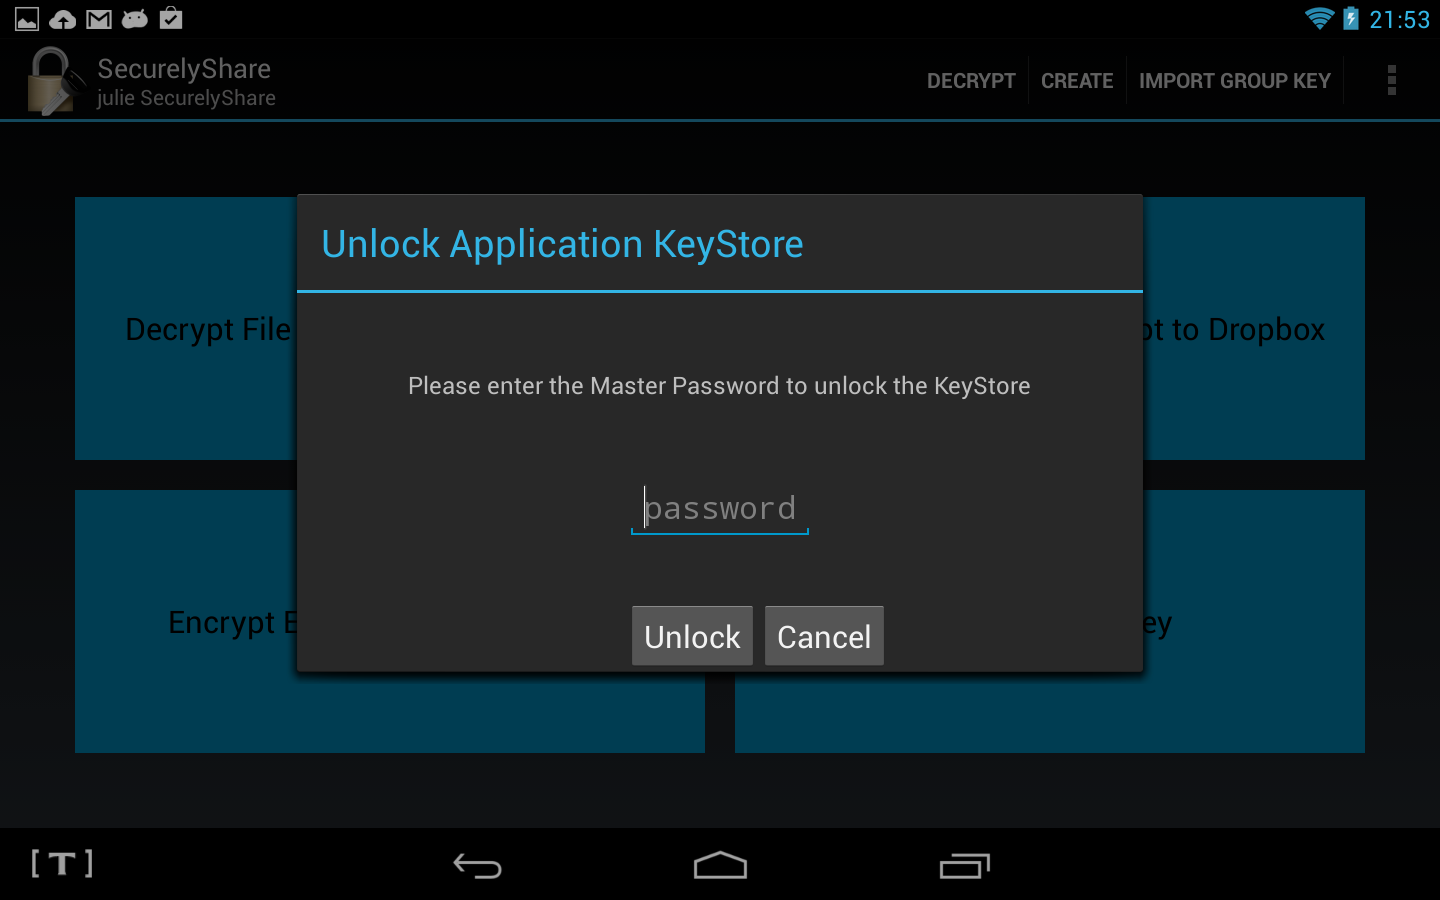
\includegraphics[width=0.6\textwidth]{Unlock}                                                                                                                                                                                                                                                                                                                                                                                                                                                                                                                                                                                                                                                                                                                                                                                                                                                                                                                                                                                                                                                                                                                                                                                                                                                                                                                                                                                                                                                                                                                                                                                                                                                                                                                                                                                                                                                                                                                                                                                                                                                                                                                                                                                                                                                                                                                                                                                                                                                                                                                                                                                                                                                                                                                                                                                                                                                                                                                                                                          
    \caption{Dialog to request Master password to unlock access to KeyStores }
    \label{fig:unlock}
\end{figure}

\subsection*{Other Features}

\subsubsection*{Fragments}

Figure \ref{fig:import} shows the screen for importing a new group key, which illustrates our use of the \texttt{Fragment} class.  

\begin{figure}[h!]
    \centering
    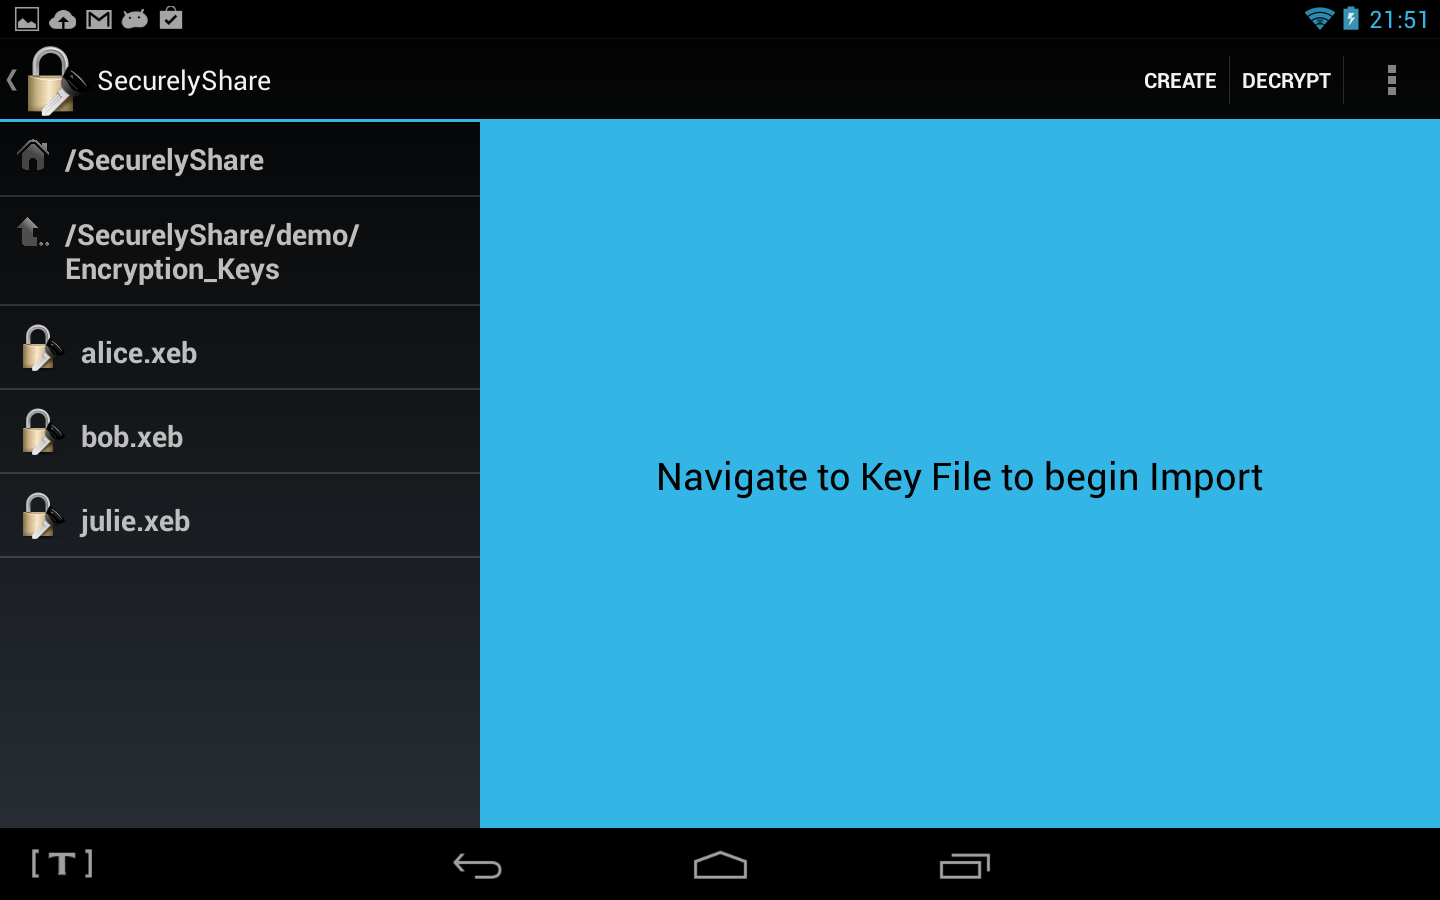
\includegraphics[width=0.6\textwidth]{import}                                                                                                                                                                                                                                                                                                                                                                                                                                                                                                                                                                                                                                                                                                                                                                                                                                                                                                                                                                                                                                                                                                                                                                                                                                                                                                                                                                                                                                                                                                                                                                                                                                                                                                                                                                                                                                                                                                                                                                                                                                                                                                                                                                                                                                                                                                                                                                                                                                                                                                                                                                                                                                                                                                                                                                                                                                                                                                                                                                          
    \caption{Import a group key }
    \label{fig:import}
\end{figure}

Fragments are reusable elements of the application's user interface which can be combined to build a multi-pane user interface \citep{androiddev3}. As shown here, SecurelyShare is perhaps  best suited to landscape mode as it uses a split-screen, however it could easily be modified to show each fragment in a separate activity on a smaller screen or to improve the display in portrait mode.

\subsubsection*{Performance and Threading}
Although some asynchronous processing results from the calls to the Dropbox API, currently everything in SecurelyShare runs on the main thread.  Whilst this may seem an unusual choice when carrying out computationally expensive cryptographic operations, there is little value in introducing parallel processing if it frees the user up to do other tasks.  When opening a file, there is little else that the user can practically do apart from wait and in testing, we felt that performance was within acceptable limits.  This may need to be revisited in a future iteration;  if, for example, a custom PDF processor was implemented where users were needing to encrypt and save large annotated files, it may be preferable to run this on a separate thread.

\section{Admin System}
\red{
Admin system – basic with no front end.  Designed to run on system with Dropbox installed and running so files uploaded to dropbox simply by saving them in the correct location rather than worrying about using Dropbox API within program.
}
\red{
PC version in java that just does basic encryption/decryption.  Used primarily for intial development and testing of encryption mechanisms. Single username hardcoded for testing. Fully developed application with user interface outside of scope of this project. Assumption that encrypted blobs are probably also created on PC - simple PC version of program developed to address this, although no gui developed
}\\

\section{Implementation Challenges}
Android is highly event-driven; its activities are written using the familiar syntax of Java and, as a new Android developer, it is easy to fall into the trap of thinking of them as 'programs'.  However, they could perhaps be more properly thought of as sophisticated event-handlers.  Android activities do not control the flow of program execution - they simply provide code to respond to events.  

We found that this different way of thinking was one of the most challenging aspects of this project - basic  concepts like opening a dialog to ask the user to confirm an action and blocking until the user responds are simply not available.  Similarly unfamiliar is the way that the operating system actively manages storage.  When the user navigates away from an activity, the operating system holds it in memory in a paused state.  If, however, memory resources run short, the current instance of the activity is simply destroyed and a new one created next time the user navigates back to it, causing variables to be reinitialised (although the system saves the state of the activity layout so that it can recreate the screen when the user resumes the application).  This uncertainty over the precise state of variables required close attention when coding. 

\subsubsection*{Communication between activities}
When wanting to start a new activity, the standard method is to create an \texttt{Intent} and then to execute \texttt{startActivity(intent)}.  Data to be passed to the new activity can be placed in a \texttt{Bundle} belonging to the intent.  However, in order to pass an object in this way it must be serializable, either using standard Java serialization or by implementing \texttt{Parcelable} , Android's own implementation which is lighterweight and faster.  In SecurelyShare we are working with object of the Dropbox API, which are neither parecelable nor serializable.  Considerable time was spent investigating whether there was an obvious solution to this which we were simply missing due to inexperience but ultimately it appeared that there was none and we had to design around this limitation.


\subsubsection*{Security Providers}
The Java SE Documentation states:
\begin{quotation}
\textbf{Reminder: }Cryptographic implementations in the JDK are distributed through several different providers ("Sun", "SunJSSE", "SunJCE", "SunRsaSign") for both historical reasons and by the types of services provided. General purpose applications SHOULD NOT request cryptographic services from specific providers. \citep{javasedoc}
\end{quotation} 
Having followed this advice, we discovered that although we were able to decrypt and import group keys in the desktop version of our code, this did not work when ported to Android.  This presented a major debugging difficulty as, having isolated the problem, we were essentially comparing two pieces of code that looked identical but performed differently.  It transpired that the problem arose because Java and Android use different default providers and these are not interchangeable.  We were able to remedy the problem by installing the Bouncy Castle provider and forcing Java to use that provider.

\red{
CHALLENGES
Major issues with keystore, certificates 
No access to key tool in android
THINGS NOT INCLUDED
However, as will be discussed in Chapter \ref{cha:imp}, due to some of the challenges encountered during the implementation phase, we were not able to implement this aspect of our design fully in the prototype. (digital signatures)
}\\




\section{Testing}

The encryption and decryption elements of our prototype were largely testing by inspection - known texts were encrypted, the files were checked to ensure that they were not leaking any of the plaintext, and these were in turn decrypted and compared with the original.   In general, the nature of encryption means that the main body of a file either decrypts completely or not at all, however particular attention must be paid to the very beginning and end of a file, as incorrect use of the API can lead to errors here.  As our project was aimed at document encryption, we tested using a mixture of text (.txt files) and PDFs (although we did also confirm that our processes generalised to other file types).  Since randomness plays an important role in ensuring  semantic security  for symmetric encryption schemes, this made any sort on unit testing extremely difficult.  At the outset we considered using fixed initialisation vectors and encryption keys to make our tests repeatable.  However, on closer consideration this involved making some significant changes to the program logic relating to the use of the cryptography APIs and so was considered to make this sort of testing meaningless.  

Other aspects of the user interface were tested manually, trying to make sure that a range of user inputs and behaviour were covered.  However, it should be noted that the prototype was not designed to be releasable code and therefore did not include comprehensive validation of user input. Although certain common scenarios were handled (for example, the user is informed if trying to decrypt a document without first importing the appropriate group key), it was deemed that for the purposes of this prototype it was acceptable that other less common behaviours should be permitted to cause the app to terminate (e.g. if the app permission is revoked via the Dropbox website whilst the app is running).  

When a user shifts focus away from the current activity, the activity is kept in memory but is switched into the background.  Such processes can be killed at any time by the system in order to reclaim memory.  In this event, when the user returns to the activity, it is recreated by the system - this may cause some expected results if not designed for properly.  Since this process is managed by the operating system and is determined by a number of external factors, it can prove difficult to test.  If testing in an emulated environment, it is possibly to simulate an artificially small device memory to encourage this behaviour to be triggered.  However, as previously mentioned, this option was not available to us so a similar effect was created by rotating the device, which also causes an activity to be recreated.  Even though not identical, it proved quite an effective substitute in our testing.

